\subsection*{Exercise 2: Controllability}

\subsubsection*{2.1 Which of these systems are stable when \( u_n = 0 \)?}

The discrete linear dynamical system \( x_{n+1} = Ax_n \) is stable if and only if the eigenvalues of the matrix \( A \) satisfy that \( | \lambda | < 1 \). So we can apply eigendiagonalization on these dynamical systems:

\quad (a)
\[
    A =
        \begin{bmatrix}
            1 & 0   & 1 \\
            0 & 1.5 & 0 \\
            1 & 0   & 0
        \end{bmatrix}
    =
        \begin{bmatrix}
            0.526  & 0  & 0.851 \\
            -0.000 & -1 & 0.000 \\
            -0.851 & 0  & 0.526
        \end{bmatrix}
        \begin{bmatrix}
            -0.618 & 0       & 0 \\
            0        & 1.5 & 0 \\
            0        & 0       & 1.618
        \end{bmatrix}
        \begin{bmatrix}
            0.526  & 0  & -0.851 \\
            -0.000 & -1 & 0.00000 \\
            0.851  & 0  & 0.526
        \end{bmatrix}
\]

\quad (b) (same as the previous one)
\[
    A =
        \begin{bmatrix}
            1 & 0   & 1 \\
            0 & 1.5 & 0 \\
            1 & 0   & 0
        \end{bmatrix}
    =
        \begin{bmatrix}
            0.526  & 0  & 0.851 \\
            -0.000 & -1 & 0.000 \\
            -0.851 & 0  & 0.526
        \end{bmatrix}
        \begin{bmatrix}
            -0.618 & 0       & 0 \\
            0        & 1.5 & 0 \\
            0        & 0       & 1.618
        \end{bmatrix}
        \begin{bmatrix}
            0.526  & 0  & -0.851 \\
            -0.000 & -1 & 0.00000 \\
            0.851  & 0  & 0.526
        \end{bmatrix}
\]

\quad (c)
\[
    A V =
        \begin{bmatrix}
            0.5 & 0    & 0.5  \\
            0   & -0.5 & -1 \\
            0   & 0    & 0.5
        \end{bmatrix}
        \begin{bmatrix}
            1 & 0 & -1 \\
            0 & 1 & 0 \\
            0 & 0 & 0
        \end{bmatrix}
    =
        \begin{bmatrix}
            1 & 0 & -1 \\
            0 & 1 & 0 \\
            0 & 0 & 0
        \end{bmatrix}
        \begin{bmatrix}
            0.5 & 0    & 0 \\
            0   & -0.5 & 0 \\
            0   & 0    & 0.5
        \end{bmatrix}
\]

\quad (d)
\[
    A =
        \begin{bmatrix}
            0.5  & 0.5   & 0   \\
            0    & -0.5  & -1  \\
            -0.1 & 0     & 0.5
        \end{bmatrix}
    =
        \begin{bmatrix}
            -0.843 & -0.840 & -0.468 \\
            -0.344 &  0.437 & 0.883  \\
            0.414  & -0.323 & -0.050
        \end{bmatrix}
        \begin{bmatrix}
            0.7 & 0      &  0 \\
            0      & 0.24 &  0 \\
            0      & 0     &  -0.44
        \end{bmatrix}
        \begin{bmatrix}
            -0.547 & -0.227 &  1.114 \\
            -0.722 & -0.488 & -1.877\\
            0.144  & 1.286  & 1.362
        \end{bmatrix}
\]

So the systems of case (a) and (b) are unstable when \( u_n = 0 \), while the systems of (c) and (d) are stable.

\subsubsection*{2.2 Which of these systems are controllable?}
The linear dynamical system \( x_{n+1} = A x_n + B u_n \) is controllable if and only if the matrix:
\[
    \begin{bmatrix}
        B & AB & A^2 B & \cdots & A^{k-1} B
    \end{bmatrix}
\]
has full row rank (where \( k \) is the size of vector \( x_n \)). In these systems, \( x_n \in \mathbb{R}^3 \), so \( k=3 \).

Thus, we can justify the controllability of each system by calculating the matrix above and testing if it has full row rank. I wrote a simple Matlab function to help me leverage the dense computation:

\begin{minted}{matlab}
    function res = is_controllable (A, B)
        T = [B, A * B, A^2 * B];
        res = rank(T) == 3;
    endfunction
\end{minted}

And test the controllability of each system with different input:

\begin{minted}{matlab}
    A1 = [ 1 0 1; 0 1.5 0; 1 0 0 ]
    B1 = [ 0; 0; 1 ]
    is_controllable(A1, B1) % ans = 0

    A2 = [ 1 0 1; 0 1.5 0; 1 0 0 ]
    B2 = [ 0; 1; 1 ]
    is_controllable(A1, B1) % ans = 1

    A3 = [ 0.5 0 0.5; 0 -0.5 -1; 0 0 0.5 ]
    B3 = [ 1; 0; 1 ]
    is_controllable(A1, B1) % ans = 1

    A4 = [ 0.5 0.5 0; 0 -0.5 -1; -0.1 0 0.5 ]
    B4 = [ 0; 1; 0 ]
    is_controllable(A1, B1) % ans = 1
\end{minted}

\begin{enumerate}[(a)]
    \item \( rank(T) = 2 \), the system is not controllable.
    \item \( rank(T) = 3 \), the system is controllable.
    \item \( rank(T) = 3 \), the system is controllable.
    \item \( rank(T) = 3 \), the system is controllable.
\end{enumerate}


\subsubsection*{2.3 For which of these systems can you find a control law \( u_n \) to stabilize the system?}

For the systems (b), (c) and (d) we can find a control law \( u_n \) to stabilize it.

We can solve the Ricatti equation by iteration to get a list of optimal control input when we have chosen the cost matrix \( Q \) and \( R \):
\[
    P = Q + A^\mathsf{T} P A + A P B {(B^\mathsf{T} P B + R)}^{-1} B^\mathsf{T} P A
\]

However, since we are only required to stabilize the system, and the systems (c) and (d) are already stable, we do can simply set \( u_n = 0 \) for them.

For system (a), I simply set \( Q = I \) and \( R = 1 \), then solve the Ricatti equation starting from \( P_{init} = Q \) (also use Matlab to leverage the computation):

\begin{minted}{matlab}
    function [P, K] = solve_ricatti (Q, R, A, B)
        P = Q; % start from Q
        counter = 0;
        u = [];
        while true
            P_new = Q + A' * P * A - A * P * B * pinv(B' * P * B + R) * B' * P * A;
            if norm(P_new - P) < 0.00001
                break;
            end
            P = P_new;
            K = pinv(R + B' * P * B) * B' * P * A;
            counter = counter + 1;
        end
    endfunction
\end{minted}

Finally the value of \( P \) converges to:
\[
    P =
    \begin{bmatrix}
        2181.29 & -1209.03 & 1359.80 \\
        -1209.03 & 673.64 & -753.58 \\
        1359.80 & -753.58 & 849.57
    \end{bmatrix}
\]

And the \( K \) can be computed with \( K = {(B^\mathsf{T} P B + R)}^{-1} B^\mathsf{T} P A \):
\[
    K =
    \begin{bmatrix}
        14.4684 & -7.0308 & 8.8399
    \end{bmatrix}
\]

For system (b), test this controller with the initial state
\( x_{init} = \begin{bmatrix}
    5 & 5 & 5
\end{bmatrix} \).

\begin{minted}{matlab}
    function [u_traj, x_traj, counter] = test_controller (A, B, K, x_init)
        u_traj = [];
        x_traj = [];
        counter = 0;
        x = x_init;
        while true
            u = -K * x;
            x = A * x + B * u
            u_traj = [u_traj, u];
            x_traj = [x_traj, norm(x)];
            counter += 1;
            if norm(x) < 0.01
                break
            end
        end
    endfunction
\end{minted}

The test result is illustrated below:
\begin{figure}[ht]
    \centering
    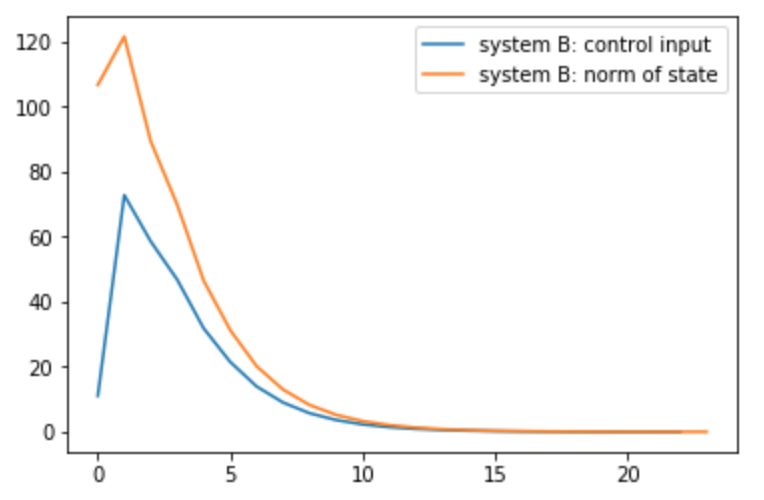
\includegraphics[width=0.5\textwidth]{imgs/p2_1.png}
\end{figure}

For system (c) and (d), test their stability when setting \( u_n = 0 \):
\begin{figure}[ht]
    \centering
    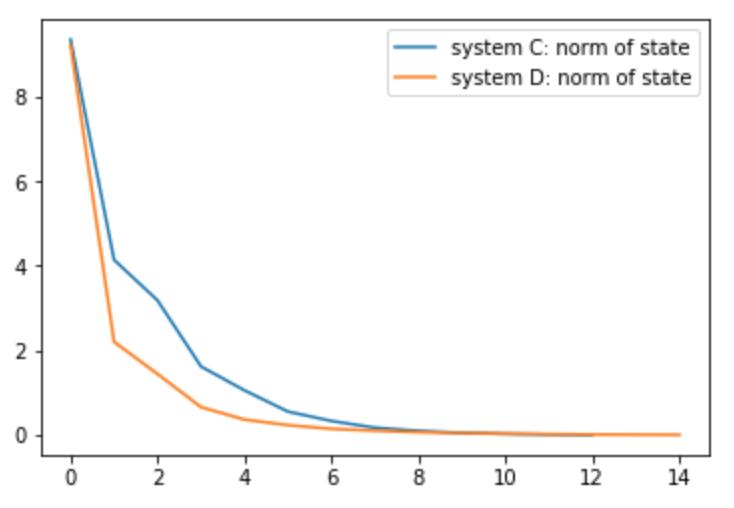
\includegraphics[width=0.5\textwidth]{imgs/p2_2.png}
\end{figure}
